\documentclass{article}

% Language setting
% Replace `english' with e.g. `spanish' to change the document language
\usepackage[english]{babel}
\usepackage{mathtools}
% Set page size and margins
% Replace `letterpaper' with `a4paper' for UK/EU standard size
\usepackage[letterpaper,top=2cm,bottom=2cm,left=3cm,right=3cm,marginparwidth=1.75cm]{geometry}

% Useful packages
\usepackage{amsmath}
\usepackage{graphicx}
\usepackage[colorlinks=true, allcolors=blue]{hyperref}

\title{Frame in quantum simulation of a driven oscillator}
\author{Tien Nguyen Dinh}

\begin{document}
\maketitle

\begin{abstract}
Your abstract \cite{greenwade93}.
\end{abstract}

\section{Introduction}

Your introduction goes here! Simply start writing your document and use the Recompile button to view the updated PDF preview. Examples of commonly used commands and features are listed below, to help you get started.

Once you're familiar with the editor, you can find various project settings in the Overleaf menu, accessed via the button in the very top left of the editor. To view tutorials, user guides, and further documentation, please visit our \href{https://www.overleaf.com/learn}{help library}, or head to our plans page to \href{https://www.overleaf.com/user/subscription/plans}{choose your plan}.

\section{The system}

For simplicity, first we consider a straightforward two-level system, or a qubit
\begin{align}
    H_0 = \frac{1}{2}\omega_q(|0\rangle\langle 0|-|1\rangle\langle 1|),
\end{align}
where $\omega_q$ is the qubit's frequency. The qubit has a dipole moment, $d=-d_0(|1\rangle\langle 0+|0\rangle\langle 1|$ and can be directly coupled to a classical field $E(t)=E_0\cos(\omega_d t + \theta)$. The interaction Hamiltonian is therefore,
\begin{align}
    H_{\text{int}}= -d\cdot E(t) &= E_0d_0\cos(\omega_d t + \theta)(|1\rangle\langle 0|+|0\rangle\langle 1|),\\
    &=\Omega_0\cos(\omega_d t +\theta)(|1\rangle\langle 0|+|0\rangle\langle 1|). 
\end{align}
We have defined $\Omega_0=E_0 d_0$. Together, the full Hamiltonian is now,
\begin{align}\label{fullH}
    H(t) &= H_0+H_{\text{int}}(t),\\
    &=\frac{1}{2}\omega_q(|0\rangle\langle 0|-|1\rangle\langle 1|)+\Omega_0\cos(\omega_d t+\theta)(|1\rangle\langle 0|+|0\rangle\langle 1|).
\end{align}

\section{Simulation in the lab frame}

We throw the whole Hamiltonian into the \texttt{sesolve} solver of QuTiP. The system's parameters are $\omega_q=10, \Omega_0=1, \omega_d=\omega_q, \theta=0$. Let us simulate from $t=0$ to $t=5$ with sampling rate $1/\texttt{nsteps}=0.001$. The results of $\langle X(t)\rangle, \langle Y(t)\rangle, \langle Z(t)\rangle$ are presented in Fig. \ref{fig:driven_twolevel}. Starting from $|0\rangle$, the system evolves unitarily according to the specified Hamiltonian. At exactly $t_g=\pi$, it reaches the second eigenstate of the $\sigma_z$ operator $|1\rangle$, indicating by $\langle Z\rangle = -1$. This is a $\pi$ gate. Note that for a driven qubit on IBM Quantum System, it is customary to vary the \textit{amplitude} $\Omega_0$ of the drive rather than the gate time $t_g$. 

Now, an important feature of the graph is the oscillatory pattern of $\langle X(t)\rangle$ and $\langle Y(t)\rangle$. At $t_0=0$ and $t_g=\pi$, they are approximately zero. However between $t_0$ and $t_g$ they oscillate rapidly between $1.0$ and $-1.0$. This indicates that the Bloch vector precesses around the $Z$ axis during evolution. Because of this precession, the Bloch vector spends some time in the state $|+\rangle$ and some time in the state $|-\rangle$. Can we get rid of this oscillatory pattern? Yes, by going to the frame rotating with the drive. Note that the drive is on resonance with the qubit $\omega_d=\omega_q$, we are in the frame of the qubit, too. 

\begin{figure}
    \centering 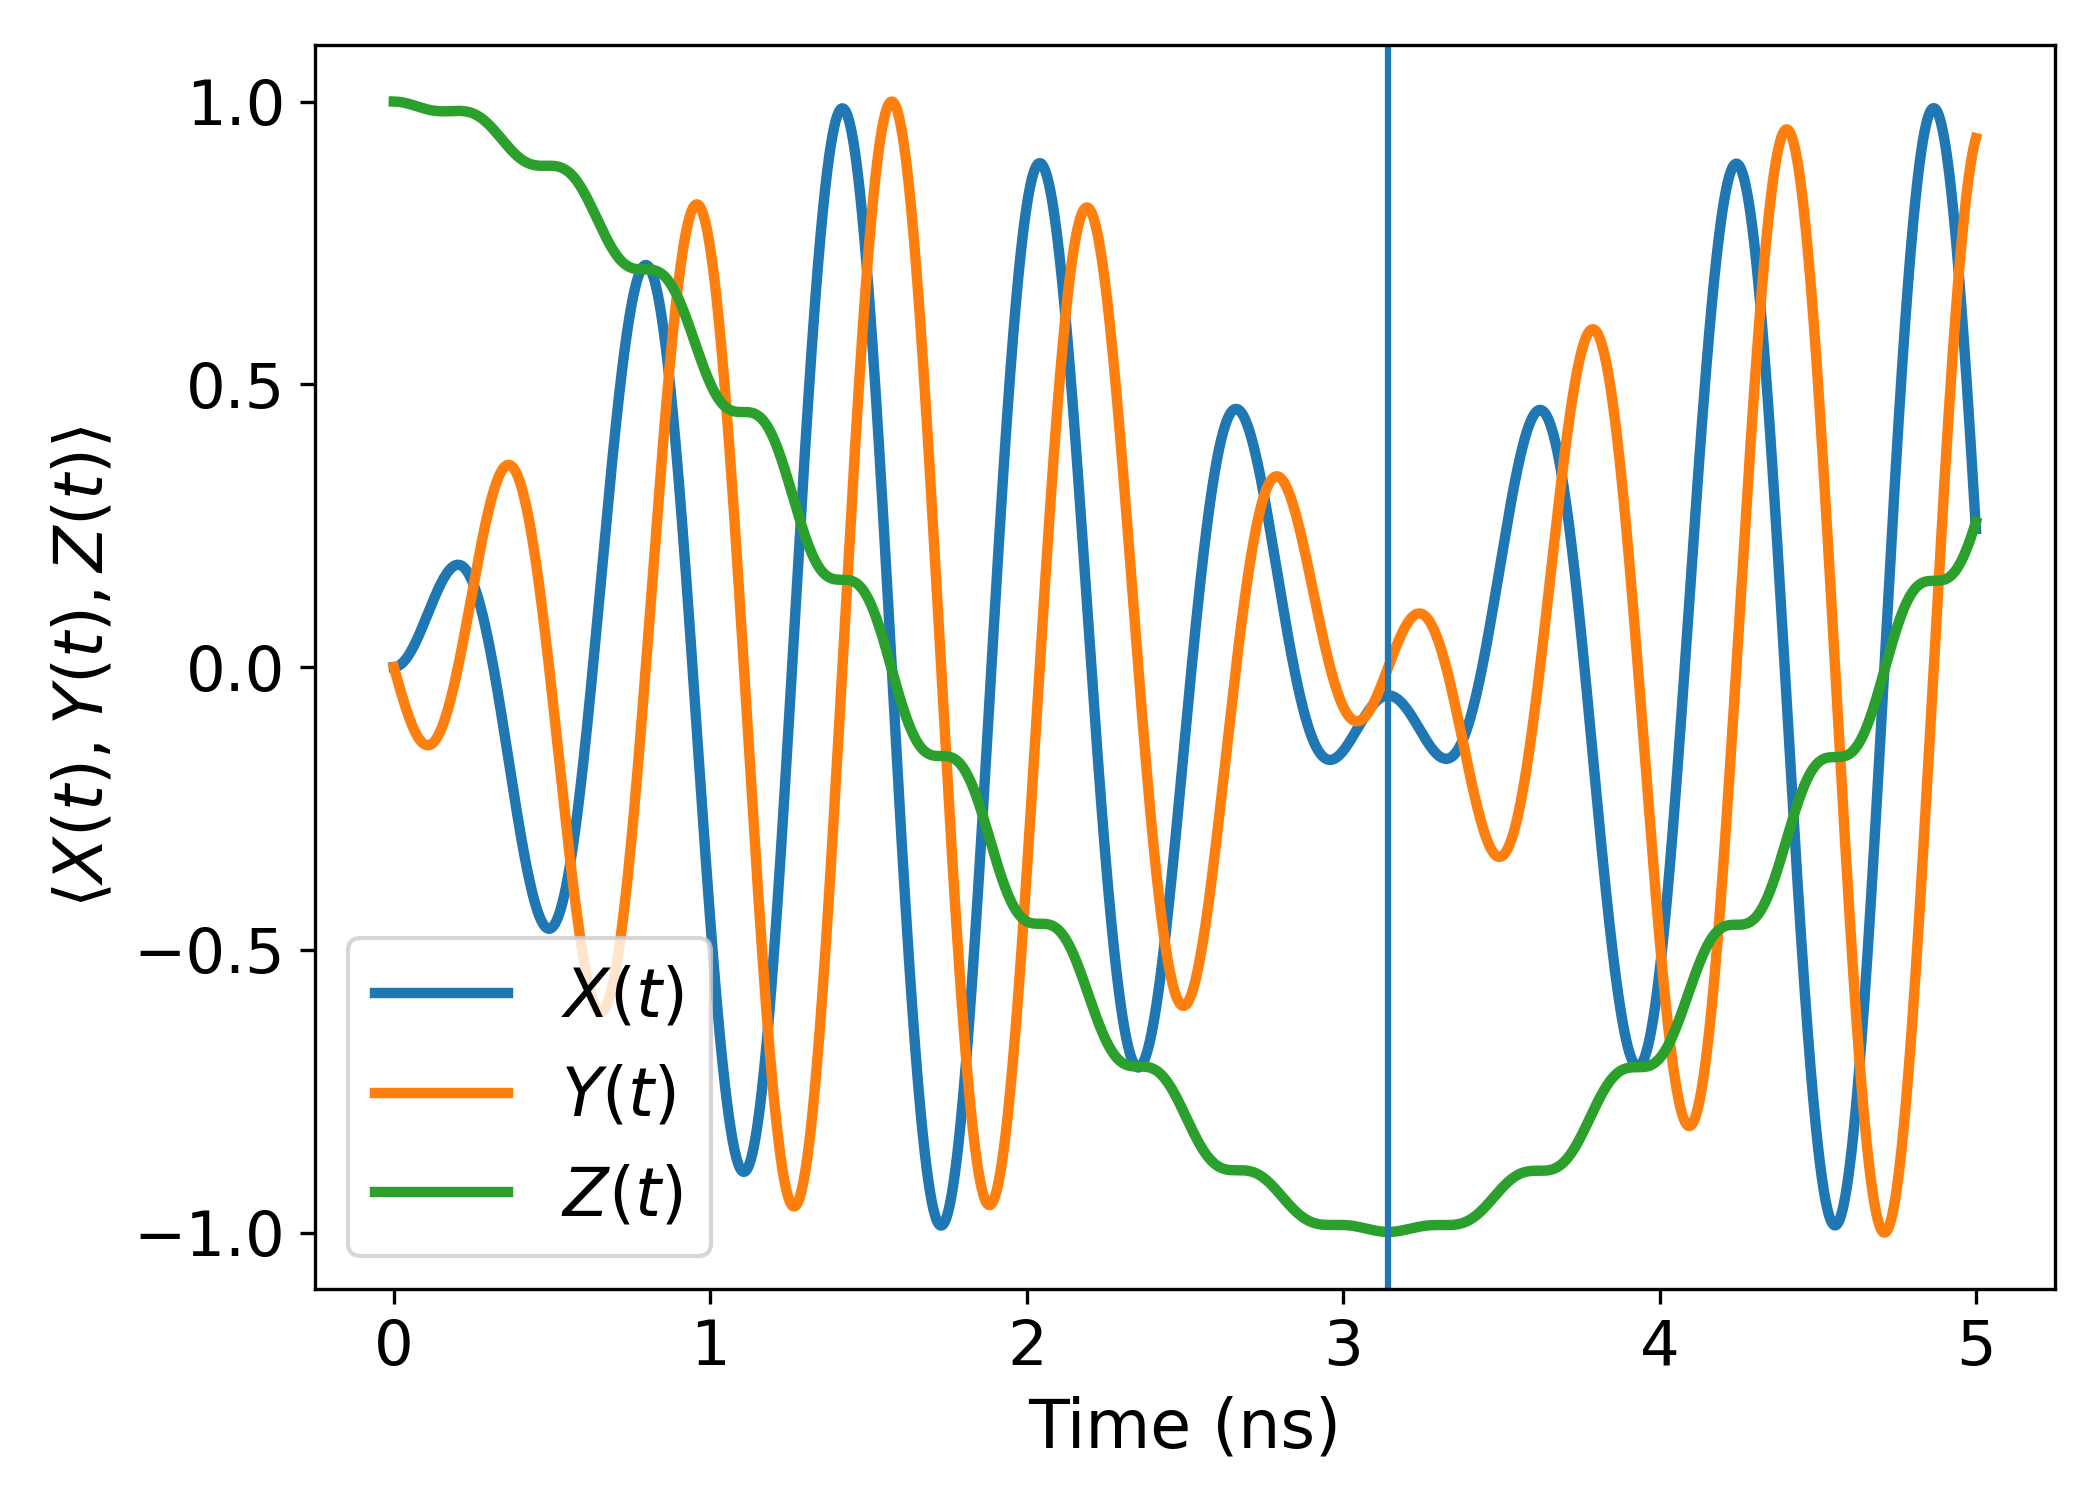
\includegraphics[scale=0.70]{driven_twolevel.png}
    \caption{Simulation of the system presented in Eqn. (\ref{fullH}). In the lab frame, the expectation values of $\langle X\rangle$ and $\langle Y\rangle$ vary with respect to time due to the precession of the Bloch vector about the $z$ axis.} 
    \label{fig:driven_twolevel}
\end{figure}

\section{Going into the drive frame}
\begin{figure}
    \centering 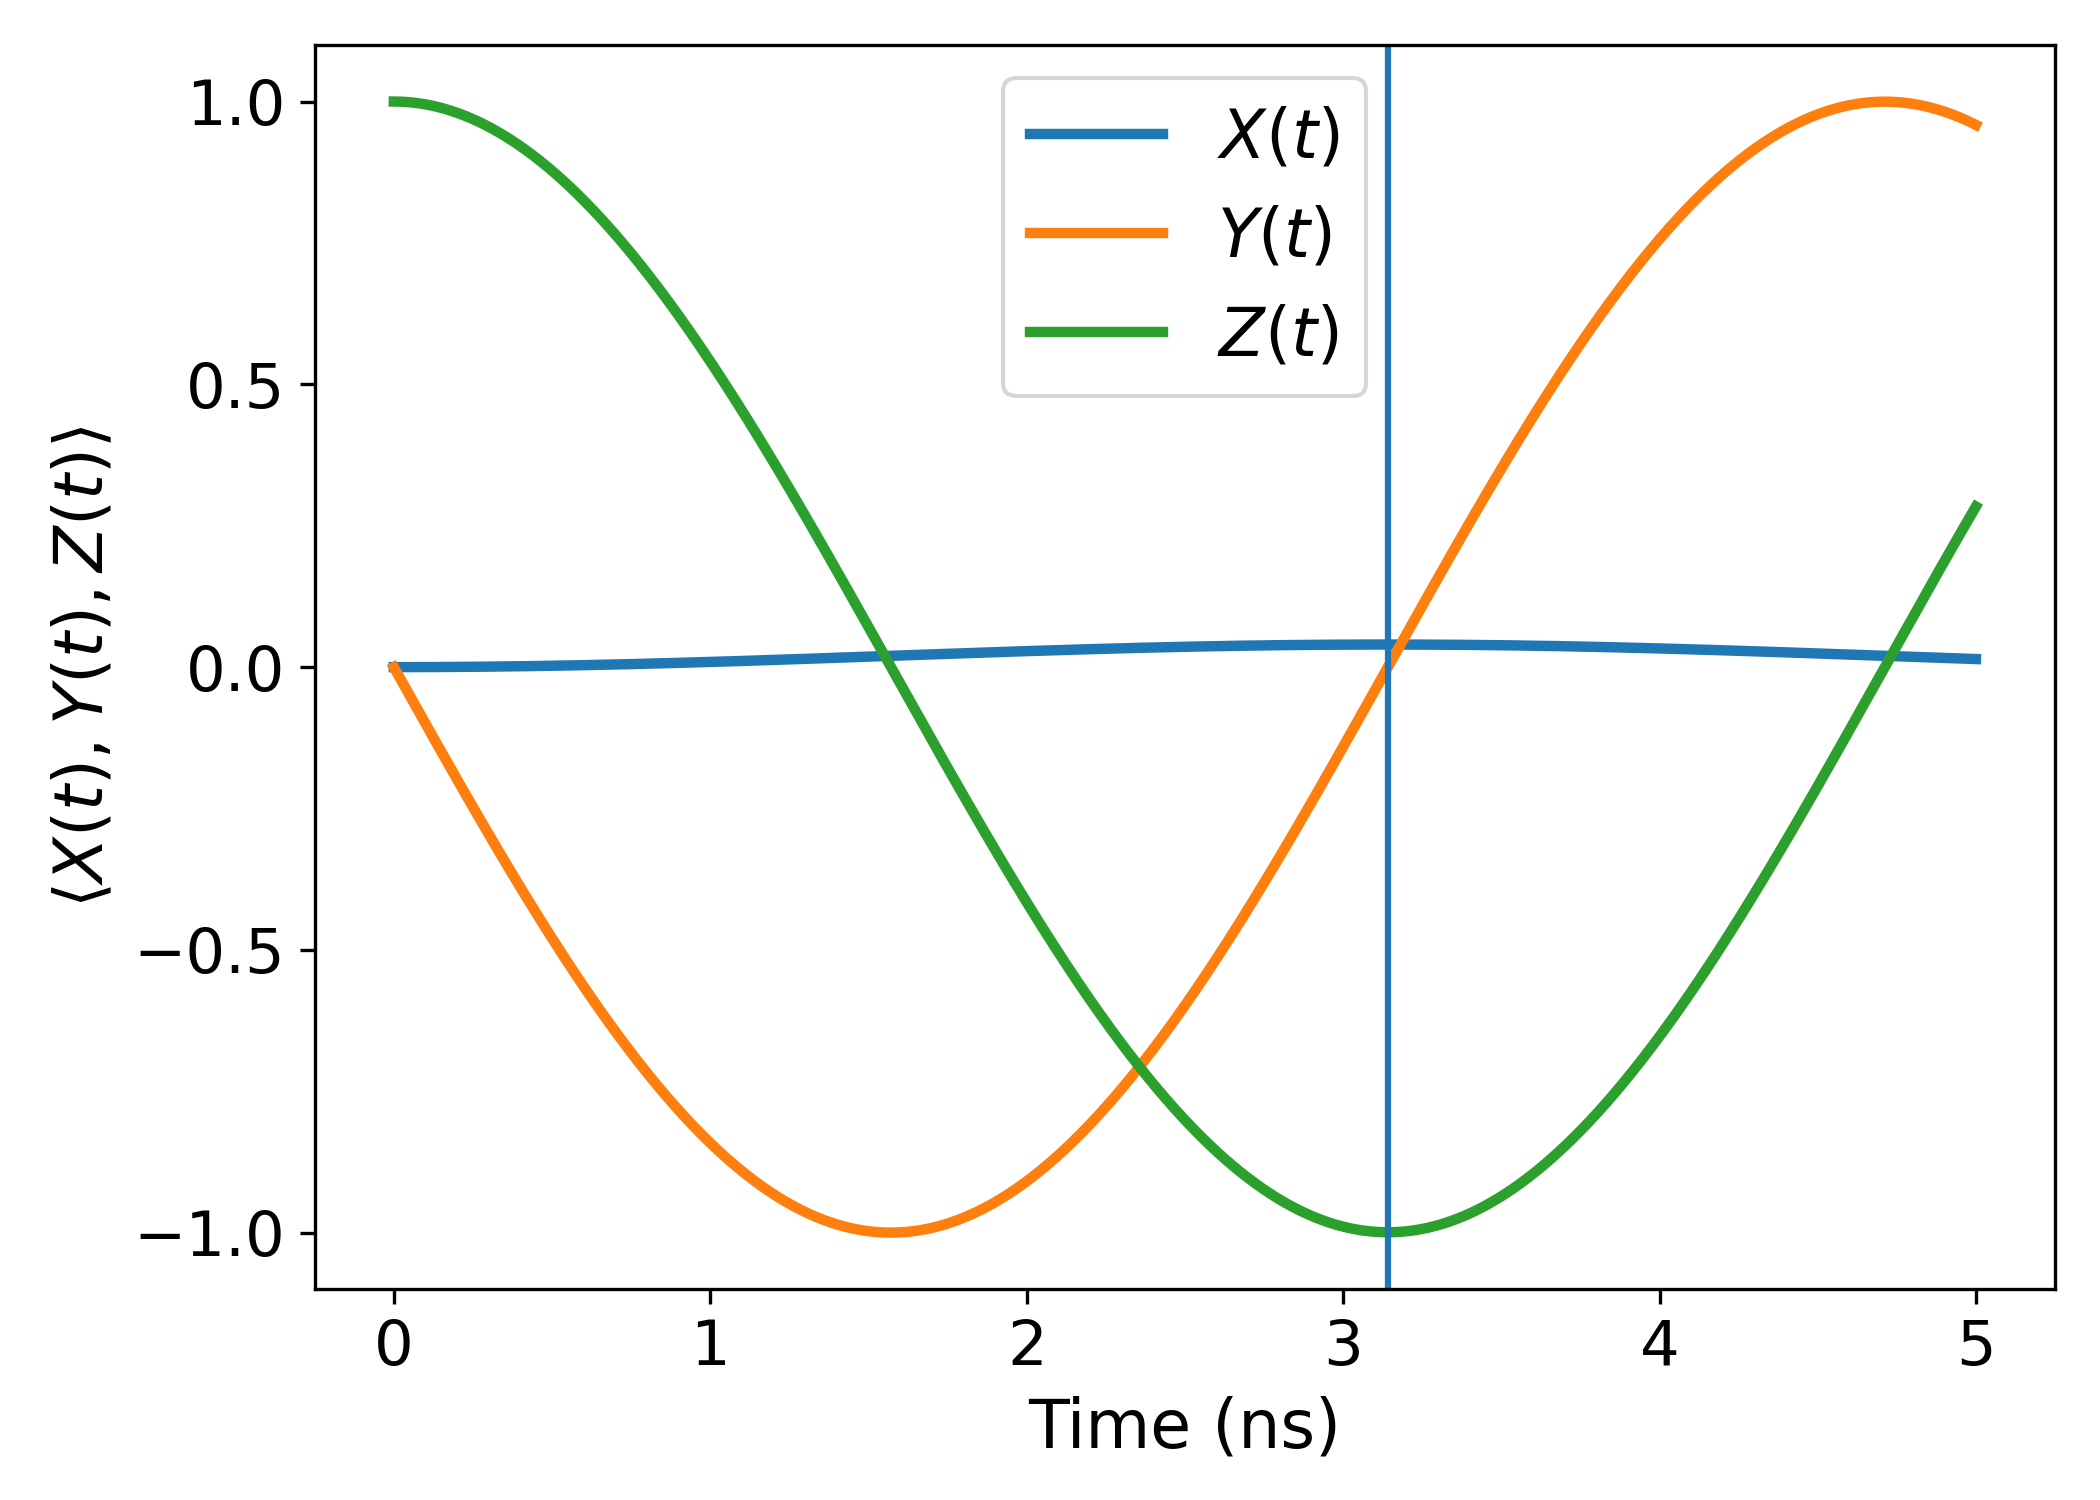
\includegraphics[scale=0.70]{driven_twolevel_drive_frame.png}
    \caption{Simulation of the system presented in Eqn. (\ref{RWAHamiltonian}). In the frame rotating with the drive frequency (nearly on resonance with the qubit's frequency) the expectation value of $\langle X\rangle$ remains $0$ throughout while that of $\langle Z\rangle$ and $\langle Y\rangle$ vary sinusoidally.} 
    \label{fig:driven_twolevel_driveframe}
\end{figure}
We start with the full Hamiltonian in the lab frame,
\begin{align}\label{fullH}
    H(t) &= H_0+H_{\text{int}}(t),\\
    &=\frac{1}{2}\omega_q(|0\rangle\langle 0|-|1\rangle\langle 1|)+\Omega_0\cos(\omega_d t+\theta)(|1\rangle\langle 0|+|0\rangle\langle 1|),\\
    &=\frac{1}{2}\omega_q \sigma_z + \left(\frac{\Omega_0}{2}e^{-i\omega_d t}+\frac{\Omega^*_0}{2}e^{i\omega_d t}\right)\sigma_x,
\end{align}
where we've switch to the Pauli basis for convenience. The drive amplitude is also re-defined to be a complex number $\Omega_0\coloneqq \Omega_0e^{-i\theta}$. Now we go into the frame specified by 
\begin{align}
    R(t) = e^{i\omega_d t\sigma_z/2}.
\end{align}
The transformed Hamiltonian reads
\begin{align}\label{RWAHamiltonian}
    H'(t)&=R^\dagger(t)H(t)R(t) + i\dot{R}^
    \dagger(t)R(t),\\
    &=\frac{\delta_{qd}}{2}\sigma_z +\dfrac{\Omega_0}{2}(\cos\theta\sigma_x + \sin\theta\sigma_y),
\end{align}
where $\delta_{qd}=\omega_q-\omega_d$. On resonance, the $\sigma_z$ term vanishes leaving only the $\sigma_x$ and $\sigma_y$ terms. The rotation axis is then completely specified by the \textit{phase} of the classical field. The Hamiltonian is now time-independent. Using the same system's parameters as above, the results of $\langle X(t)\rangle, \langle Y(t)\rangle, \langle Z(t)\rangle$ are plotted in Fig. (\ref{fig:driven_twolevel_driveframe}). In the frame rotating with the drive frequency (nearly on resonance with the qubit's frequency) the expectation value of $\langle X\rangle$ remains $0$ throughout while that of $\langle Z\rangle$ and $\langle Y\rangle$ vary sinusoidally. Note that $\theta=0$, so we're rotating about the $x$-axis. Since we're rotating about the $x$-axis, we expect that the Bloch vector spend some time in the middle (when $t=\pi/2$) to be in the $|+\rangle$ state. Because there's a slight detuning, the $\langle X\rangle$ line is not entirely straight throughout the evolved time. 

\subsection{Good luck!}

We hope you find Overleaf useful, and do take a look at our \href{https://www.overleaf.com/learn}{help library} for more tutorials and user guides! Please also let us know if you have any feedback using the Contact Us link at the bottom of the Overleaf menu --- or use the contact form at \url{https://www.overleaf.com/contact}.

\bibliographystyle{alpha}
\bibliography{refs}

\end{document}